%%=============================================================================
%% Methodologie
%%=============================================================================

\chapter{\IfLanguageName{dutch}{proof-of-concept}{proof-of-concept}}%
\label{ch:proof-of-concept}

In dit hoofdstuk wordt de implementatie van de proof-of-concept uiteengezet. Er zal een Space Invaders-spel worden ontwikkeld voor AllPhi, dat zij kunnen gebruiken of repliceren als een interactieve uitdaging tijdens evenementen. 

Het spel zal de vorm aannemen van een eenvoudig videospel waarin de speler diverse basisfunctionaliteiten kan uitvoeren, zoals bewegen, schieten, punten verdienen, enzovoort. Alvorens de implementatie aan te vangen, wordt een visuele representatie van het beoogde spel gecreëerd. Hiervoor dient het originele Space Invaders-spel als referentiekader.

Binnen het spel zullen verschillende typen vijanden aanwezig zijn, evenals bunkers waarachter de speler dekking kan zoeken. Daarnaast zal een willekeurig gegenereerde UFO periodiek aan de linkerkant van het scherm verschijnen, waarna deze zich naar rechts beweegt terwijl er op de speler wordt geschoten. Alle vijanden kunnen worden vernietigd, wat de speler punten oplevert. De hoeveelheid punten die de speler verdient, is afhankelijk van de positie van de vijand binnen de verschillende lagen: hoe hoger de laag, des te meer punten worden toegekend.

\section{Doelstelling}
De proof of concept heeft als doelstelling een space-invaders videospel te implementeren in Godot met gebruik makend van C\# als de scripttaal voor de engine. Hierdoor weet Allphi of het mogelijk is en zouden ze het kunnen recreëren.

\section{Implementatie}
Het spel is ontwikkeld in de Godot-engine met behulp van de programmeertaal C\#. Om aan de slag te gaan, dient u eerst de Godot-engine te downloaden van de officiële website. Er zijn twee verschillende versies beschikbaar. De standaardversie is geschikt indien u gebruik wilt maken van de ingebouwde scripttaal GDScript, een functionele programmeertaal. De alternatieve versie biedt ondersteuning voor C\#.
\\
Na het downloaden en uitpakken van de engine zijn er geen verdere installatiestappen vereist, in tegenstelling tot sommige andere engines. Bij het openen van Godot worden verschillende panelen gepresenteerd.
\\
Bij het aanmaken van een nieuw project in Godot kan men kiezen uit drie verschillende renderers. De eerste, genaamd "Compatibility", is geschikt voor eenvoudige 2D-videospellen en biedt betere speelbaarheid op oudere apparaten. Deze renderer maakt gebruik van OpenGL 3 als backend en heeft minder geavanceerde 3D-graphics, wat voor de huidige usecase geen belemmering vormt aangezien er een 2D-spel wordt ontwikkeld.
\\
De tweede renderer, "Mobile", is ontworpen voor de ontwikkeling van videogames voor mobiele apparaten en desktops. Deze biedt verbeterde rendering voor eenvoudigere spellen, vergelijkbaar met de "Compatibility"-renderer. Een nadeel is dat complexere scènes minder schaalbaar zijn met deze renderer.
\\
De derde en laatste optie, "Forward+", is uitsluitend geschikt voor desktop-platformen en is bedoeld voor de ontwikkeling van 3D-videospellen. Deze renderer is geschikt voor het creëren van complexe spellen.

Gezien de specifieke usecase is de "Mobile"-renderer geselecteerd voor de implementatie van het spel.
\\
Na het creëren van een nieuw project wordt het bovenstaande scherm gepresenteerd. Dit scherm bestaat uit verschillende panelen, elk met een specifieke functie. Aan de rechterzijde bevindt zich het scènepaneel, waarin alle nodes worden weergegeven die zich in de huidige scène bevinden. Daaronder is het assets-paneel te vinden, waar alle grafische elementen, zoals afbeeldingen en sprites, worden opgeslagen. Een node kan worden opgeslagen als een scène, waardoor deze herbruikbaar wordt en in het assets-paneel verschijnt. Aan de rechterzijde van het scherm worden de eigenschappen van de momenteel geselecteerde node getoond.

\section{Eindresultaat}
Het eindresultaat is te zien aan de onderstaande foto. De github repository is te vinden via deze link: \url{https://github.com/BramLippens/Godot-CSharp-Space-Invaders}
\begin{figure}[h]
    \centering
    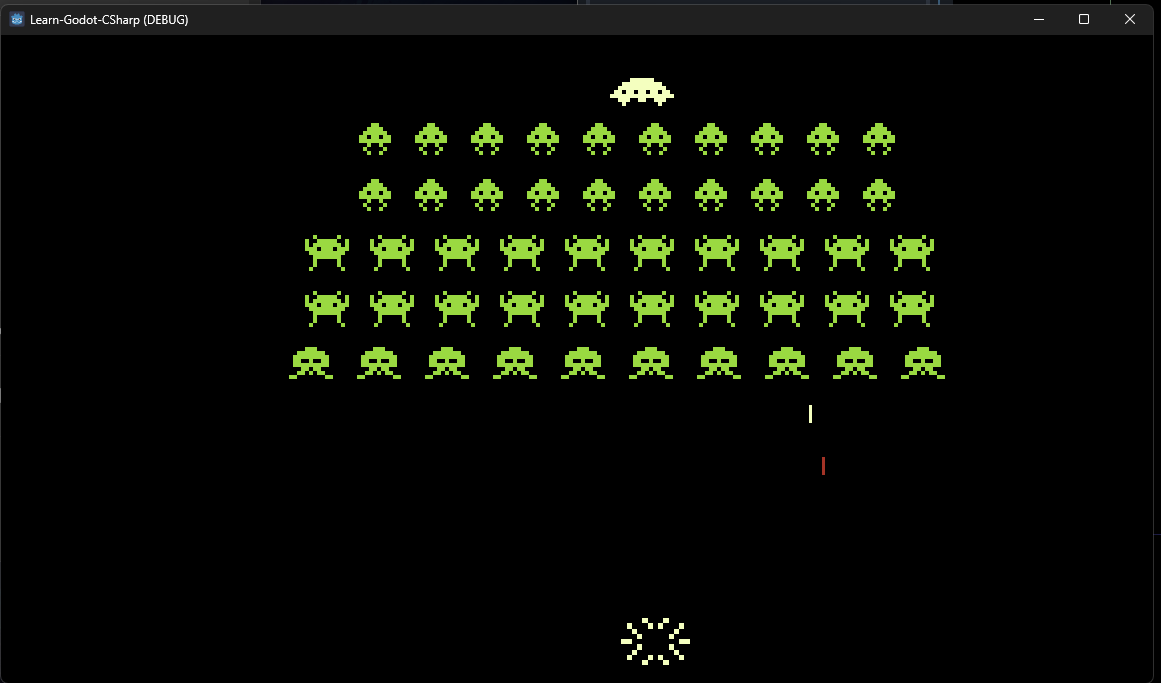
\includegraphics[width=1\textwidth]{ImplementatieSpel.png}
    \caption{Implementatie}
    \label{fig:POC}
\end{figure}

